The Precision Timed ARM (PTARM) architecture is a realization of the PRET principles on an ARM ISA architecture\todo{Citation}. 
In this chapter we will describe in detail the implementation details of the timing-predictable ARM processor and discuss the worst-case execution time analysis of code running on it.
We show that with the architectural design principles of PRET, the PTARM architecture is easy analyzable with repeatable timing.
  
The architecture of PTARM closely follows the principles discussed in chapter~\ref{chapter:pret}.
This includes a thread-interleaved pipeline with scratchpads along with the timing predictable memory controller.
The ARM ISA was chosen not only for its popularity in the embedded community, but also because it is a Reduced Instruction Set Computer(RISC), which has simpler instructions that allow more precise timing analysis. 
Complex Instruction Set Computers(CSIC) on the other hand adds un-needed complexity to the hardware and timing analysis.
RISC architectures typically features a large uniform register file, a load/store architecture, and fixed-length instructions.
In addition to these, ARM also contains several unique features.
ARM's ISA requires build a single cycle hardware shifter along with an arithmetic logic unit(ALU), as all of its data-processing instructions can shift its operands before passed onto the ALU. 
ARM's load/store instructions also contain auto-increment capabilities that can increment or decrement the base address. 
This is useful to compact code that is reading through an array in a loop, as one instruction can load the contents and prepare for the next read in one instruction.
In addition, almost all of the ARM instructions are conditionally executed.
The conditional execution improves architecture throughput with potential added benefits of code compaction\todo{Citation}.     
ARM programmer's model specifies 16 registers (R0 to R15) to be accessed with its instructions, with register 15 being the program counter. 
Any data-operation done on register 15 triggers a branch.  

ARM has a rich history of versions for their ISA, and PTARM implements the ARMv4 ISA, currently without support for the thumb mode.
PTARM uses scratchpads instead of caches, and a DDR2 DRAM for main memory managed by the timing predictable memory controller.
PTARM includes hardware support for several floating point operations, and implements the timing instructions introduced in chapter~\ref{chapter:programming_models}.   
We will first discuss the architectural details of PTARM, then present the C++ software simulator of PTARM.   
   
\section{PTARM Architecture}
\begin{figure}
  \vspace{-20pt}
  \begin{center}
    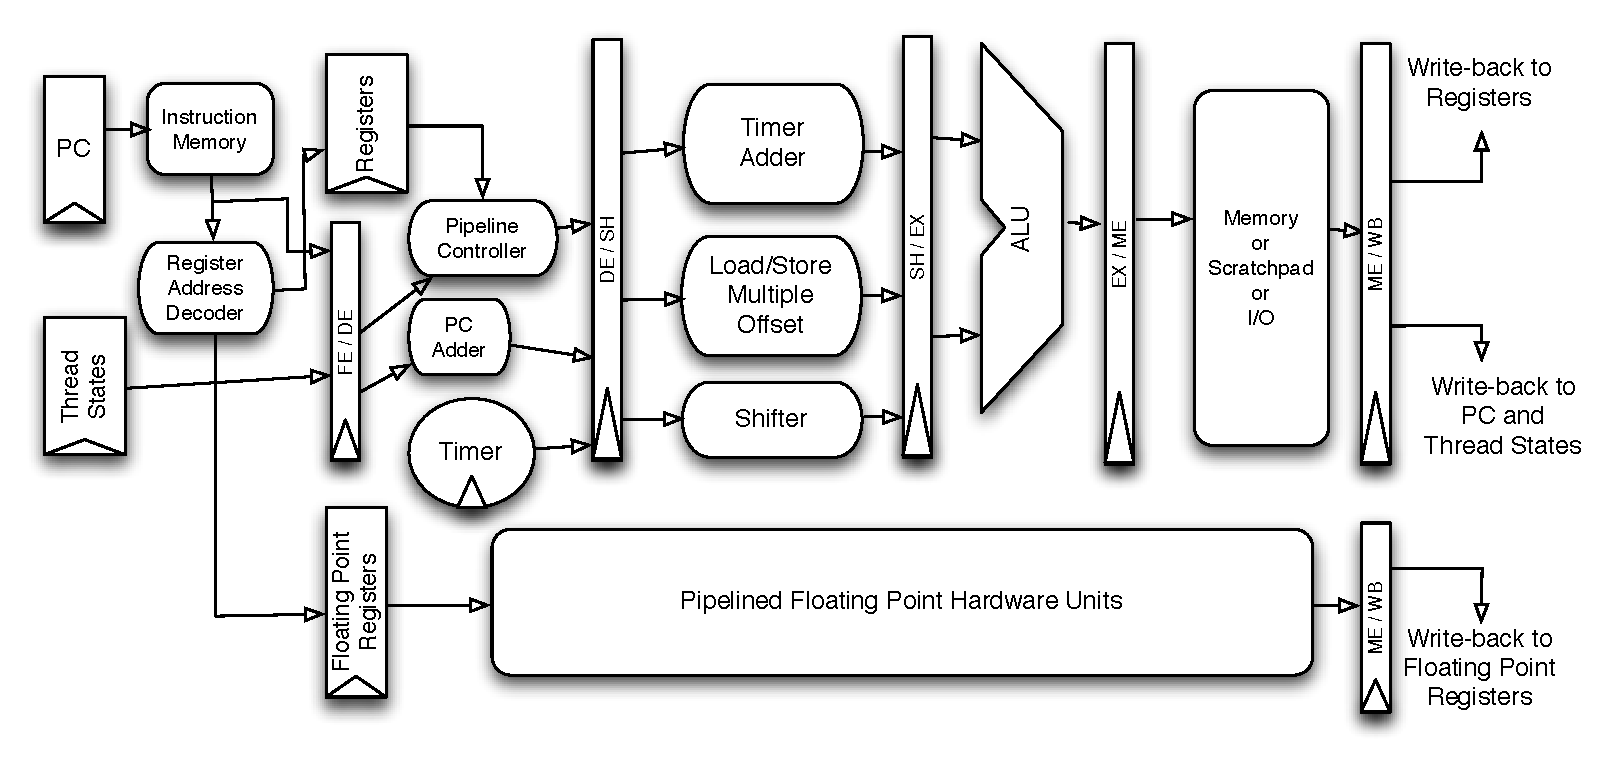
\includegraphics[scale=.6]{figs/ptarm_pipeline}
  \end{center}
  \vspace{-20pt}
  \caption{Block Level View of the PTARM pipeline}
  \label{fig:ptarm_pipeline}
\end{figure}

The pipeline of PTARM implements a thread-interleaved pipeline for the ARM instruction set.
PTARM is written in VHDL and targets Xilinx Virtex-5 Family FPGAs, thus a the design decisions made tailored the PTARM architecture towards optimizing the design for the Xilinx V5 FPGA.
It has a 32 bit datapath and consists of a six stage pipeline and can support a minimum of six threads interleaving through the pipeline.
The pipeline can be clocked up to $180MHz$ on a Virtex-5 lx110t FPGA.  
Figure~\ref{fig:ptarm_pipeline} shows a block diagram view of the pipeline. 
The multiplexers within the pipeline have been omitted in the figure for a simplified view of the hardware components that make up the pipeline.
There contains multiple copies of the Program Counter(PC), Thread States, and Register File, which are not shown in the figure.
Most of the pipeline design follows a typical Hennesy and Patterson\todo{citation} 5 stage pipeline, but the thread interleaved pipeline also allows us to strip away the branch predictor and the data forwarding logic used to handle data-hazards.
The six stages in the pipeline are -- Fetch, Decode, Shift, Execute, Memory, Writeback.
We will briefly describe the functional blocks of each stage, and later show how most instruction types are implemented in the pipeline.  
%TODO: Talk about register file, 3 read and 1 write port

The fetch stage of the pipeline selects the correct PC according to which thread is executing, and passes the address to instruction scratchpad.
A simple $Log(n)$ bit upcounter is used to keep track of which thread current to fetch.  
At this point we assume the source code fits entirely on the instruction scratchpad.
Later when we present the memory hierarchy of PTARM we will discuss further about the implications of larger code bases.
Once the instruction is received from the scratchpad, it goes through a register address decoder to quickly determine what bits to send to the register.
Typical RISC instruction sets such as MIPS have encoding of instruction bits where the register operands have a fixed location for all instruction types.
Thus, once the instruction is received from instruction memory, the selected bits can be propagated as addresses to the register file. 
In the ARM instruction set however, not all instruction encoding have the register addresses at the same location. 
Thus, we insert in a simple and small logic block for a quick decoding of register addresses.
%Todo: Add more description of the logic block? 

The decode stage of the pipeline consists of the pipeline controller which does the full decoding of instructions and sets the correct pipeline signals to be propagated down the pipeline. 
Typically the controller needs to know the current instructions in the pipeline to detect the possibility of pipeline hazards.
However,in a thread-interleaved pipeline, other instructions in the pipeline belong to other threads, thus the controller logic is greatly simplified. 
It simply decodes the instruction to determine the correct signals to send to the data-path and multiplexers down the pipeline. 
These signals get propagated down the pipeline stages, and they control the execution units to ensure the correct actions are taken, and signal the multiplexers to select the correct data operands.  
Because most of ARM instructions are conditionally executed, the pipeline controller also checks the condition bis to determine whether the instruction is to be executed or not.  
The PC Adder is almost just a simple adder that increments the PC. 
The only addition is instead only outputting an address incremented by four, it outputs two addresses, the PC incremented by both four and eight. 
The address calculation of ARM branch instructions add the offset to PC+8, instead of just the current PC, so we need to store the additional PC offset of eight in case of branch instructions.
The Timer logic block is a hardware counter clocked to the processor clock which is used to implement the timing instructions mentioned in chapter~\ref{chapter:programming_models}.
The Timer counts time in nanoseconds, and it's hardware logic does not reside in the decode stage. 
The time value however is latched in the decode stage as the subsequent stages use it for timer manipulation, so in figure~\ref{fig:ptarm_pipeline} we include it in the decode stage.
We will discuss in more detail how the timing instructions are implemented later in this chapter. 

The shift stage of the pipeline is the additional stage on top of a conventional five stage pipeline. 
The ARM ISA data-processing instructions include shifter bits and even a shifter operand for data-processing register shift instructions to shift the operands before the logical or arithmetic operations.
Thus, an extra 32 bit shifter is included to shift the operands before the execution stage. 
The Load/Store Multiple Offset logic block is used to calculate the offset of load/store multiple instructions.
The load/store multiple instruction uses a 16 bit vector to represent each of the 16 general purpose registers.
The bits that are set in that bit vector represents a load/store on that register.
The an offset is added to the base memory address for the instruction, and that offset depends on how many bits are set. 
Thus, the load/store multiple offset logic block does a bit count on the bit vector and adjusts the offset to be passed into the ALU for load/store multiple instructions.
We will later describe in detail how the load/store multiple instructions are executed within the pipeline.
The timer adder logic block is a 32 bit add/subtract unit. 
Since time is represented in 64 bit values, we add an additional 32 bit add/subtract-er so the execution stage doesn't need to incorporate a 64 bit ALU.

The execute stage simply just contains the 32 bit ALU that can do both logical and arithmetic operations. 
The memory stage interacts with the data scratchpad and memory controller, and the write back stage writes the correct data back to the registers and hardware thread states.

The floating point hardware units are pipelined floating point computation units generated with the Xilinx Coregen tool. 
 
%TODO: Memory Hierarchy
\section{Instruction Implementations}
In this section we will go into more details about how each instruction type is implemented and how the hardware blocks shown in the previous sections are used.
We will go through different instruction types and also discuss the timing implications of our implementation. 
We will summarize with a table with all instructions and the cycle count it takes to execute them.   
\subsection{Data-Processing}

\subsection{Branch}
\begin{figure}
  \vspace{-20pt}
  \begin{center}
    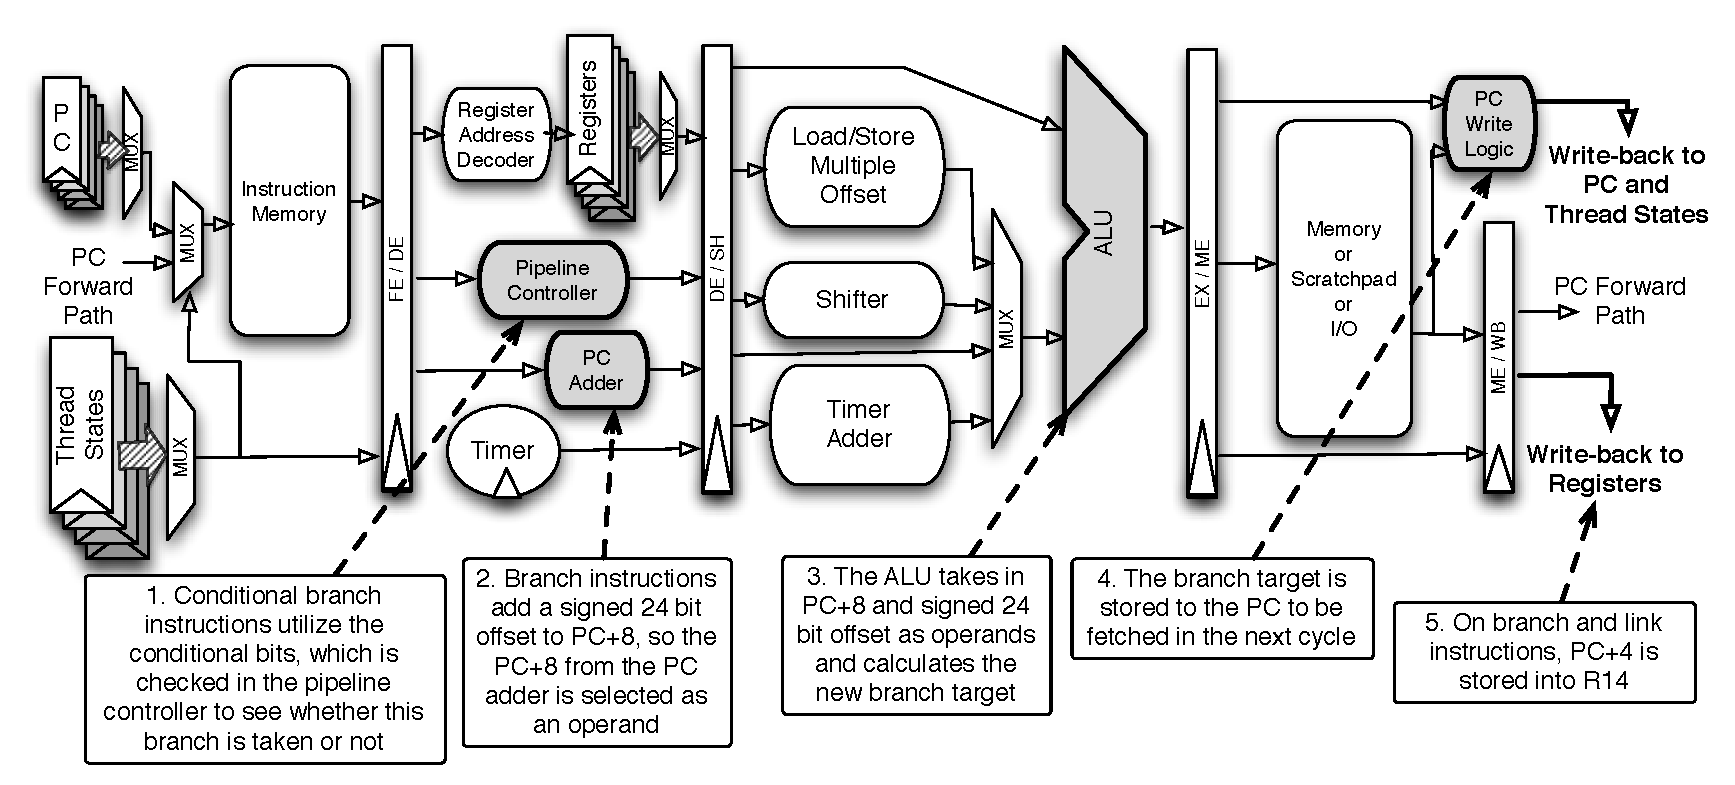
\includegraphics[scale=.6]{figs/branch_pipeline_implementation}
  \end{center}
  \vspace{-20pt}
  \caption{Branch Instruction Execution in the Ptarm Pipeline}
  \label{fig:branch_pipeline_implementation}
\end{figure}
Branch instructions in the ARM can conditionally branch forward or backwards by up to 32MB. 
Because the general purpose register 15 is the PC, any write to R15 is also considered a branch instruction that branches to the address written into R15.
Figure~\ref{fig:branch_pipeline_implementation} show how the branch instruction is executed in the thread-interleaved pipeline. 
The hardware units involved are highlighted in gray and the lines are in bold.
The branch instructions for the ARM ISA calculate the address based upon an offset added to PC incremented by 8. 
Thus, the PC adder, in addition to incrementing the PC by 4, also increments the PC by 8 to pass to the ALU for correct address calculation. 
Once the address is calculated, it is written back to the PC for the corresponding thread.
If the instruction is a branch and link ($bl$), PC+4 will be written back to the link register (R14).   
In the case of a conditional branch, the PC is only written back if the condition holds true, or else PC+4 is written back to the PC. 
Because of the thread interleaved pipeline, we are not concerned that the pipeline will be stalled waiting for result of the branch to execute the next instruction. 
Instead, instructions from other threads will be fetched before the results of the branch is needed.     
Thus, we can write back to the PC at the end of the pipeline without creating hazards.
\subsection{Loads and Stores}
\begin{figure}
  \vspace{-20pt}
  \begin{center}
    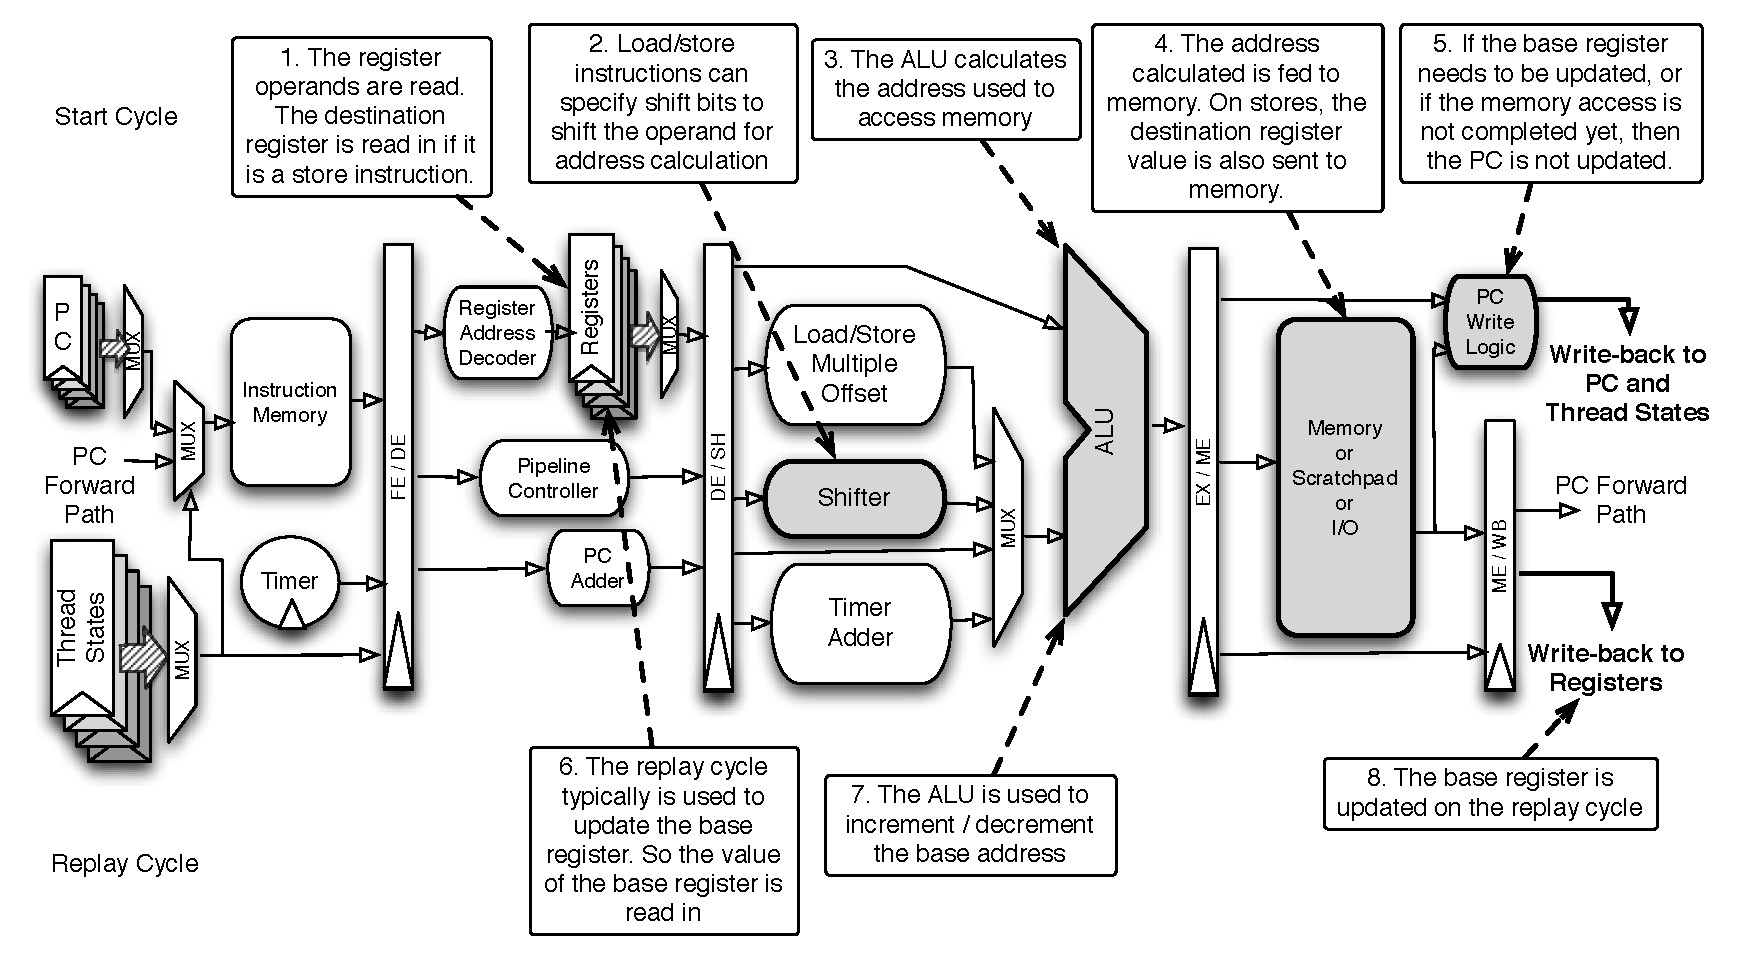
\includegraphics[scale=.6]{figs/ldstr_pipeline_implementation}
  \end{center}
  \vspace{-20pt}
  \caption{Load/Store Instruction Execution in the Ptarm Pipeline}
  \label{fig:ldstr_pipeline_implementation}
\end{figure}
For load and store instructions, the memory access address is formed by combining a base register and an offset value. 
ARM also specifies the ability to update the base register after any memory operation. 
This compacts code that reads arrays, as a load or store instruction can access memory and updates the base register so the next memory access is done on the updated base register.
ARM calls these pre-indexed and post-indexed addressing modes. 
Pre-indexed addressing mode calculates the memory address by first using the value of the base register and offset, then updating the base register. 
Post-indexed addressing mode first updates the base register, then uses the updated base register value along with the offset to form the memory address. 
The base register could be incremented or decremented when it is being updated.   
Because there is only one write port to our register file however, we cannot simultaneously write back a load result from memory and the updated base register to the register file in a single cycle. 
As a result, 
\subsection{Floating Point}

\subsection{Timing Instructions}

\section{PTARM Simulator}
\label{sec:ptarm_sim}

\section{Worst Case Execution Time Analysis}
\label{sec:wcet}




